%% Figure from MATH 556 notes, section 43 (Lecture 18). From the board sketch (Lecture 18).
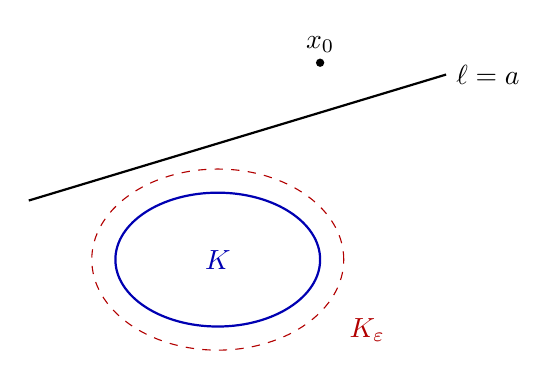
\begin{tikzpicture}[scale=1.0, >=stealth]
    \draw[thick, blue!70!black] (0,0) ellipse (1.3 and 0.85);
    \node[blue!70!black] at (0,0) {$K$};
    \draw[dashed, red!70!black] (0,0) ellipse (1.6 and 1.15);
    \node[red!70!black, anchor=west] at (1.55,-0.9) {$K_\varepsilon$};
    \draw[thick] (-2.4,0.75) -- (2.9,2.35) node[right] {$\ell = a$};
    \fill (1.3,2.5) circle (1.5pt) node[above] {$x_0$};
\end{tikzpicture}
